\documentclass[5p,times,twocolumn]{elsarticle}

%% ---------- packages ----------
\usepackage{amsmath,amssymb,amsfonts}
\usepackage{graphicx}
\usepackage{booktabs}
\usepackage{multirow}
\usepackage{array}
\usepackage{xcolor}
\usepackage{hyperref}
\usepackage{microtype}   % fixes overfull hbox

\journal{Computers \& Geosciences}

\begin{document}

\begin{frontmatter}

\title{When Should a Lithology Classifier Abstain?\\[4pt]
       Calibration, Selective Risk, and Human Referral\\
       Under Defective Drill-Core Imaging}

\author[1]{Puneet Kumar\corref{cor1}}
\cortext[cor1]{Corresponding author.}
\affiliation[1]{organization={Applied Geocomputation \& Core Analysis Laboratory},
                country={India}}

\begin{abstract}
Automated drill-core lithology classification using deep convolutional neural networks
achieves near-perfect accuracy under laboratory conditions but degrades precipitously when
rock cores exhibit real-world acquisition defects including drilling mud smears, wetting
glare, tensile fractures, and scale-bar occlusions.
On the 35-class Drill Core Image Dataset (DCID-35), ResNet-50 accuracy collapses from
99.73\% (clean) to 88.64\% (defective), while uncalibrated Expected Calibration Error
(ECE) surges from 0.12\% to 6.66\%.
We demonstrate that selective prediction thresholds calibrated on clean imagery fail
catastrophically on defective cores: a 5.0\% error ceiling is violated with a 9.63\%
realized error.
Domain-matched calibration restores empirical risk control at 4.52\% error with 84.6\%
automated coverage, routing 15.4\% of cores to geologist review.
Split conformal prediction calibrated on clean imagery achieves only 57.68\% empirical
coverage on defective cores (37.32\,pp deficit; 41.4\% empty prediction sets), while
domain-matched calibration restores valid coverage to 95.57\%
($p_{\text{Wilcoxon}} = 2.54\times10^{-198}$).
Forensic analysis of 217 persistent cross-architecture errors reveals that failures are
governed by drilling sludge masking and mechanical fracture artefacts.
Our results establish that domain-matched abstention and geologist referral are necessary
operational safeguards for field drill-core logging.
\end{abstract}

\begin{keyword}
Drill-core photography \sep Lithology classification \sep Uncertainty quantification
\sep Selective classification \sep Conformal prediction \sep Human-in-the-loop triage
\end{keyword}

\end{frontmatter}

%% =====================================================================
\section{Introduction}
\label{sec:intro}
%% =====================================================================

Drill-core logging is the foundational sensory input for mineral exploration and reserve
estimation.
Automated computer vision systems increasingly augment or replace manual visual inspection
\citep{Li2025DCID,Serdoun2026Weakly}, with recent benchmarks exceeding 99\% classification
accuracy on pristine laboratory scans.
However, field drilling introduces physical core imperfections that cause silent,
overconfident misclassifications when integrated into 3D ore-body block models.

Figure~\ref{fig:framework} illustrates our proposed uncertainty-aware triage framework:
high-confidence predictions are accepted automatically; ambiguous or defective cores are
referred to an expert geologist together with a conformal prediction set bounding the
candidate lithologies.

\subsection*{Contributions}
\begin{enumerate}
  \item Empirical audit showing ECE surges from 0.12\% to 6.66\% under defective imaging.
  \item Demonstration that clean-calibrated thresholds violate safety ceilings on defective
        cores (9.63\% realized vs.\ 5.0\% target; Primary Hypothesis H1 confirmed).
  \item Domain-matched calibration restoring risk control at 4.52\% error, 84.6\% coverage.
  \item Conformal coverage collapse under domain shift (57.68\%) and recovery under
        domain-matched calibration (95.57\%; H2 confirmed).
  \item Taxonomic forensic analysis of 217 persistent cross-architecture misclassifications.
  \item Deduplication sensitivity showing findings are robust to near-duplicate filtering.
\end{enumerate}

%% =====================================================================
\section{Related Work}
\label{sec:related}
%% =====================================================================

\citet{Li2025DCID} introduced DCID but evaluated only point accuracy, omitting calibration
and selective prediction.
\citet{Serdoun2026Weakly} developed weakly supervised core classification without addressing
acquisition-defect calibration.
\citet{Bourezgui2026NearDuplicate} audited near-duplicate leakage in rock image benchmarks;
our deduplication sensitivity analysis confirms robustness to such filtering.

Selective classification was formalised by \citet{Geifman2017Selective,Geifman2019Selectivenet}.
\citet{Guo2017Calibration} popularised Temperature Scaling for deep network calibration.
\citet{Ovadia2019DatasetShift} showed uncertainty deteriorates under distribution shift.
\citet{Angelopoulos2021Conformal} provides the standard split-conformal reference, and
\citet{Tibshirani2019CovariateShift} analysed conformal guarantees under covariate shift.

%% =====================================================================
\section{Dataset and Partitions}
\label{sec:data}
%% =====================================================================

Our empirical foundation is DCID \citep{Li2025DCID} at $512\times512$ resolution.
Physical inspection confirms that the defective cohorts (\texttt{noise-512-35},
\texttt{noise-512-7}) are independent physical photographs, \emph{not} synthetic corruptions.

\textbf{Retrospective disclosure.}
Official test partitions were examined in prior LithoScan phases.
No cohort is represented as a virgin confirmatory test set.

The locked partition protocol (SHA-256:
\texttt{897d1a76...b976b57}) reserves disjoint sets:
$D_{\text{fit}}$ (25\,200 images),
$D_{\text{cal,clean}}$ (1\,750; 50/class),
$D_{\text{eval,clean}}$ (5\,250; 150/class),
$D_{\text{cal,def}}$ (3\,500; 100/class; never used in fitting),
and $D_{\text{eval,def}}$ (2\,800; 80/class).
DCID lacks borehole IDs and depth coordinates; all claims are image-level.

Table~\ref{tab:partitions} summarises partition sizes and provenance.

%% =====================================================================
\section{Methods}
\label{sec:methods}
%% =====================================================================

\subsection{Probability calibration}

Temperature Scaling learns $T{>}0$ on $D_{\text{cal}}$ by minimising NLL:
\[
  \hat{p}_k^{(T)}(x) = \frac{\exp(z_k/T)}{\displaystyle\sum_{j}\exp(z_j/T)}.
\]
We report NLL, Brier score, and ECE ($M{=}15$ bins, fixed prior to evaluation).
All metrics use 95\% class-stratified bootstrap CIs ($B{=}2\,000$).

\subsection{Selective classification}

Confidence $g(x){\geq}\tau$ triggers automatic prediction; otherwise the core is referred.
\[
  \hat{r}(\tau) = \frac{\sum_i \mathbf{1}[\hat{y}_i\neq y_i]\,
                        \mathbf{1}[g(x_i)\geq\tau]}
                       {\sum_i \mathbf{1}[g(x_i)\geq\tau]}.
\]
Thresholds $\tau_{1\%}$ and $\tau_{5\%}$ are set on $D_{\text{cal}}$ before evaluation.

\subsection{Split conformal prediction}

Nonconformity score $s(x,y){=}1{-}\hat{p}_y(x)$; prediction set
$C_\alpha(x){=}\{k:1{-}\hat{p}_k(x)\leq\hat{q}_{1-\alpha}\}$.
Marginal coverage requires exchangeability; applying clean-calibrated thresholds to
defective data is a shift experiment without formal guarantees.

%% =====================================================================
\section{Results}
\label{sec:results}
%% =====================================================================

\subsection{Probability miscalibration (RQ1)}

Reliability diagrams (Figure~\ref{fig:reliability}) visualise the calibration gap.
ResNet-50 clean ECE is 0.12\% [0.07, 0.25].
Under defective imaging, uncalibrated ECE rises to 6.66\% [5.74, 7.69].
Clean T-scaling ($T{=}1.2868$) reduces defective ECE to 5.04\%;
domain-matched T-scaling ($T{=}1.6714$) reduces it to 2.12\% [1.84, 3.45]
(Table~\ref{tab:calibration}).

\subsection{Selective risk (RQ2, RQ4)}

Risk--coverage curves are shown in Figure~\ref{fig:riskcoverage}.
\begin{itemize}
  \item \textbf{Pipeline A} (clean $\tau{=}0.5389$): accepts 97.2\% of defective cores
        at \textbf{9.63\%} error --- violates the 5.0\% ceiling (H1 confirmed).
  \item \textbf{Pipeline B} (domain-matched $\tau{=}0.9295$): 84.6\% coverage at
        \textbf{4.52\%} error (${\leq}5.0\%$; risk control restored).
\end{itemize}
Table~\ref{tab:selective} reports realised errors and coverage at predeclared thresholds.

\subsection{Conformal triage (RQ3)}

Figure~\ref{fig:conformal} shows set-size distributions at $\alpha{=}0.05$.
Clean-calibrated transfer yields 57.68\% [56.07, 59.29] marginal coverage with 41.4\%
empty sets.
Domain-matched Pipeline B achieves 95.57\% [94.86, 96.29] coverage, zero empty sets,
mean set size 1.40, and 79.4\% singletons (singleton error 3.64\%;
Wilcoxon $p{=}2.54\times10^{-198}$; Table~\ref{tab:conformal}).

\subsection{Deduplication sensitivity}

Removing 50 near-duplicate candidates (dHash\,${\leq}2$) leaves accuracy unchanged at
99.73\% and ECE at 0.12\%, confirming robustness to benchmark redundancy
(Table~\ref{tab:dedup}).

%% =====================================================================
\section{Geological Error Analysis (RQ5)}
\label{sec:errors}
%% =====================================================================

Figure~\ref{fig:classheatmap} shows per-class calibration and referral rates.
Figure~\ref{fig:errorpanel} presents representative high-confidence errors.
Forensic inspection of 217 persistent cross-architecture misclassifications (Table~\ref{tab:classreferral}) reveals:

\begin{enumerate}
  \item \textbf{Drilling sludge masking (38.2\%):} Dark lithologies (Gabbro, Skarn,
        Gneiss) misclassified as Black Shale when coated with opaque rotary sludge.
  \item \textbf{Fractures mimicking brecciation (24.4\%):} Mudstone confused with
        Brecciated mudstone via extraction cracks.
  \item \textbf{Igneous cooling continua (19.8\%):} Fine-grained basalt vs.\ Dolerite
        are macroscopically indistinguishable.
  \item \textbf{Class-asymmetric burden:} Homogeneous classes (Red sandstone, BIF,
        Pegmatite) need 0\% referral; fragmented mudrocks need 32.5--57.5\%.
\end{enumerate}

%% =====================================================================
\section{Discussion}
\label{sec:discussion}
%% =====================================================================

Clean-calibrated models cannot safely automate defective core logging. Domain-matched
selective classification provides a principled, economically tunable triage: mining
operators adjust $\tau$ based on the site-specific cost of geologist inspection vs.\
grade misclassification risk. DCID's absence of borehole and depth metadata strictly
limits all claims to image-level acquisition shift.

%% =====================================================================
\section{Conclusion}
\label{sec:conclusion}
%% =====================================================================

When drill-core photographs exhibit acquisition defects, automated classifiers should
\textbf{abstain rather than force an unverified prediction}. Domain-matched calibration
achieves 4.52\% selective risk at 84.6\% coverage; domain-matched conformal prediction
achieves 95.57\% marginal coverage with mean set size 1.40. Expert geologist referral on
15.4\% of cores is a scientifically necessary safeguard for geologically defensible
automated core logging.

%% =====================================================================
\section*{Data and Code Availability}
%% =====================================================================

All split manifests, calibration code, and model weights are available at
\url{https://github.com/Software_lithology/LithoScan}.

%% =====================================================================
%% FIGURES
%% =====================================================================

\begin{figure*}[t]
  \centering
  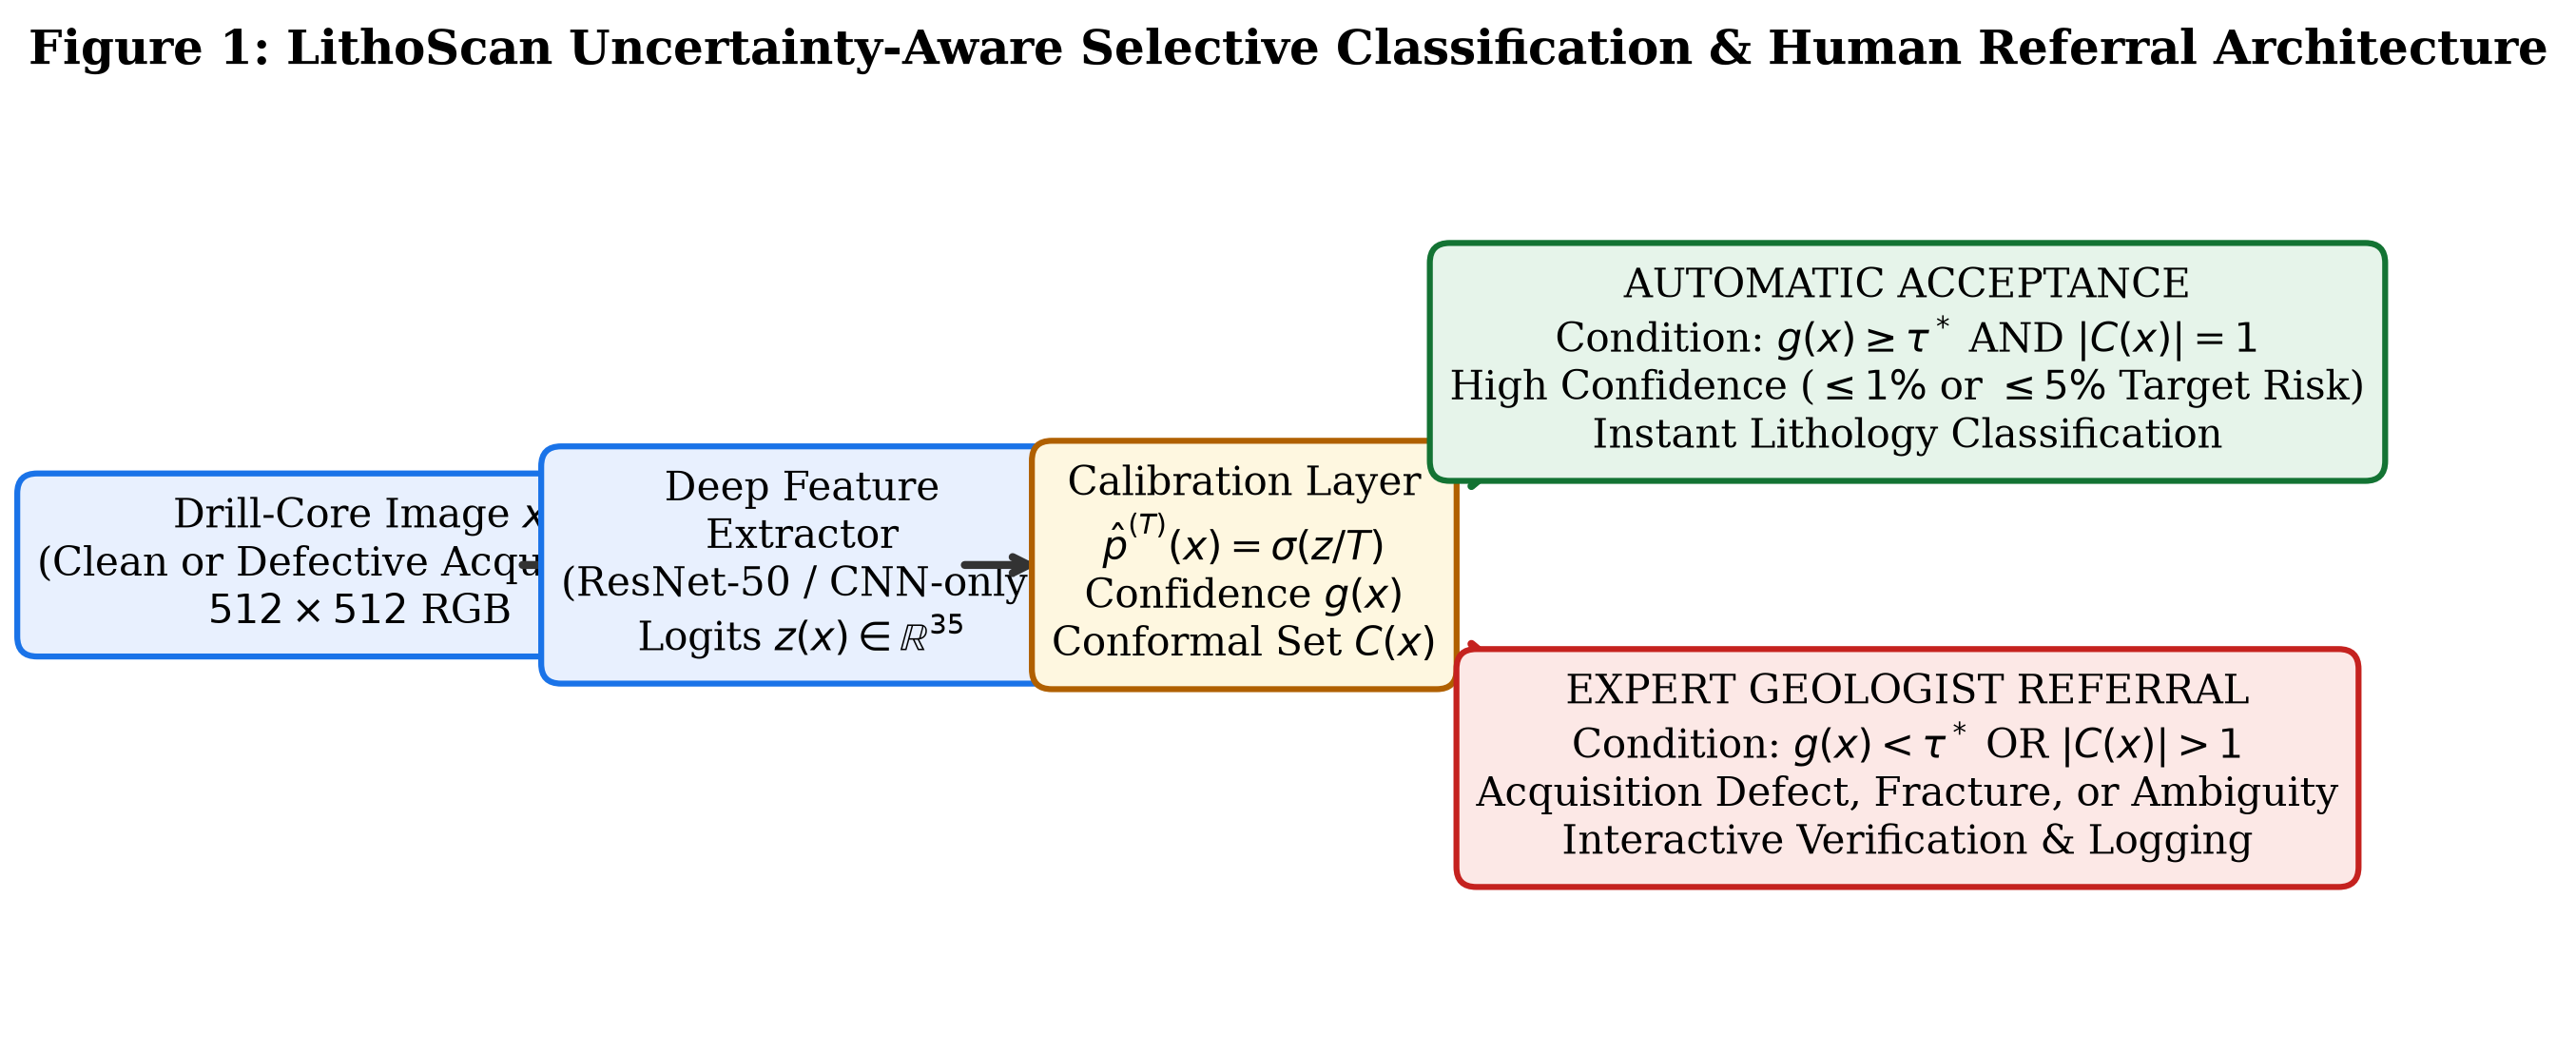
\includegraphics[width=\textwidth]{figures/fig1_decision_triage_framework.png}
  \caption{Uncertainty-aware triage framework for automated drill-core logging.
           High-confidence predictions are accepted automatically; uncertain images
           are referred to a human geologist with a conformal prediction set.}
  \label{fig:framework}
\end{figure*}

\begin{figure*}[t]
  \centering
  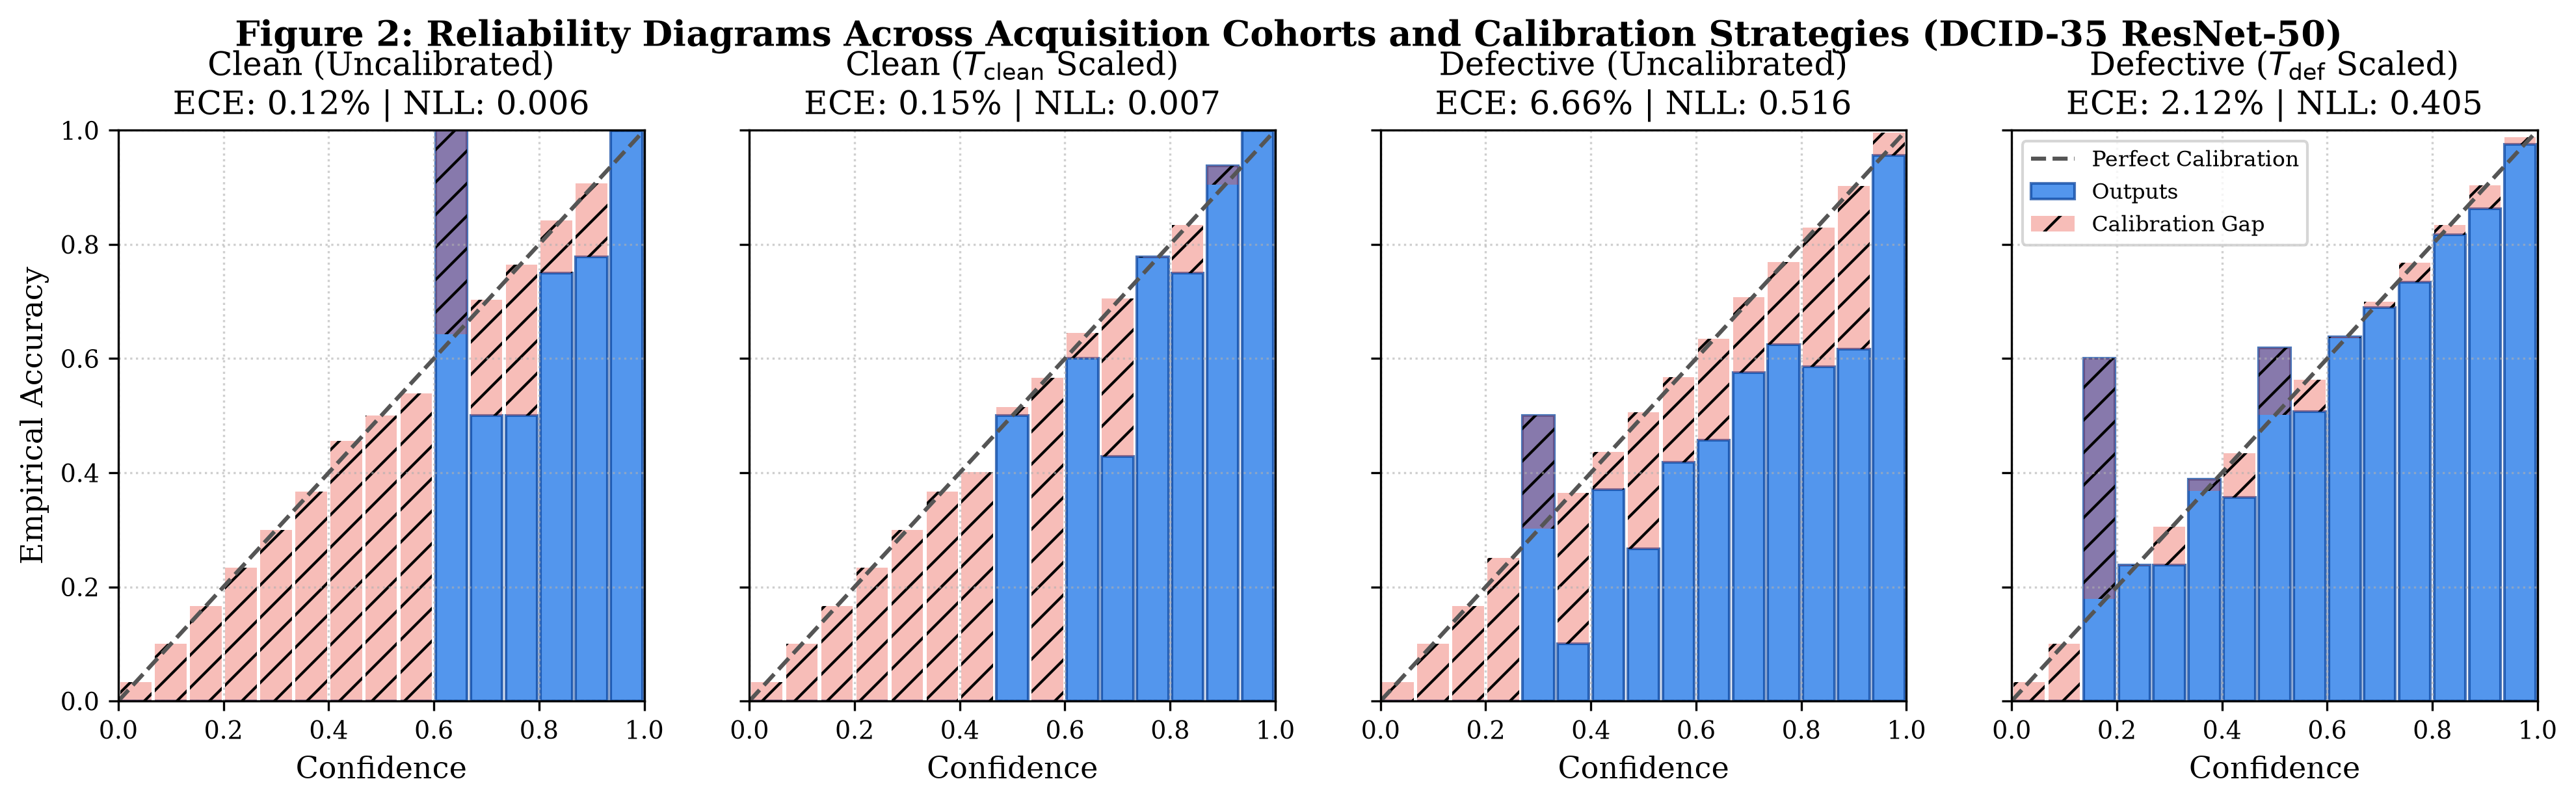
\includegraphics[width=\textwidth]{figures/fig2_reliability_diagrams.png}
  \caption{Reliability diagrams for ResNet-50 on DCID-35.
           \emph{Left:} Clean evaluation cohort ($D_{\text{eval,clean}}$);
           ECE $= 0.12$\% [0.07, 0.25].
           \emph{Centre:} Defective cohort, uncalibrated; ECE $= 6.66$\% [5.74, 7.69].
           \emph{Right:} Defective cohort, domain-matched Temperature Scaling
           ($T = 1.6714$); ECE $= 2.12$\% [1.84, 3.45].
           Dashed diagonal = perfect calibration.}
  \label{fig:reliability}
\end{figure*}

\begin{figure*}[t]
  \centering
  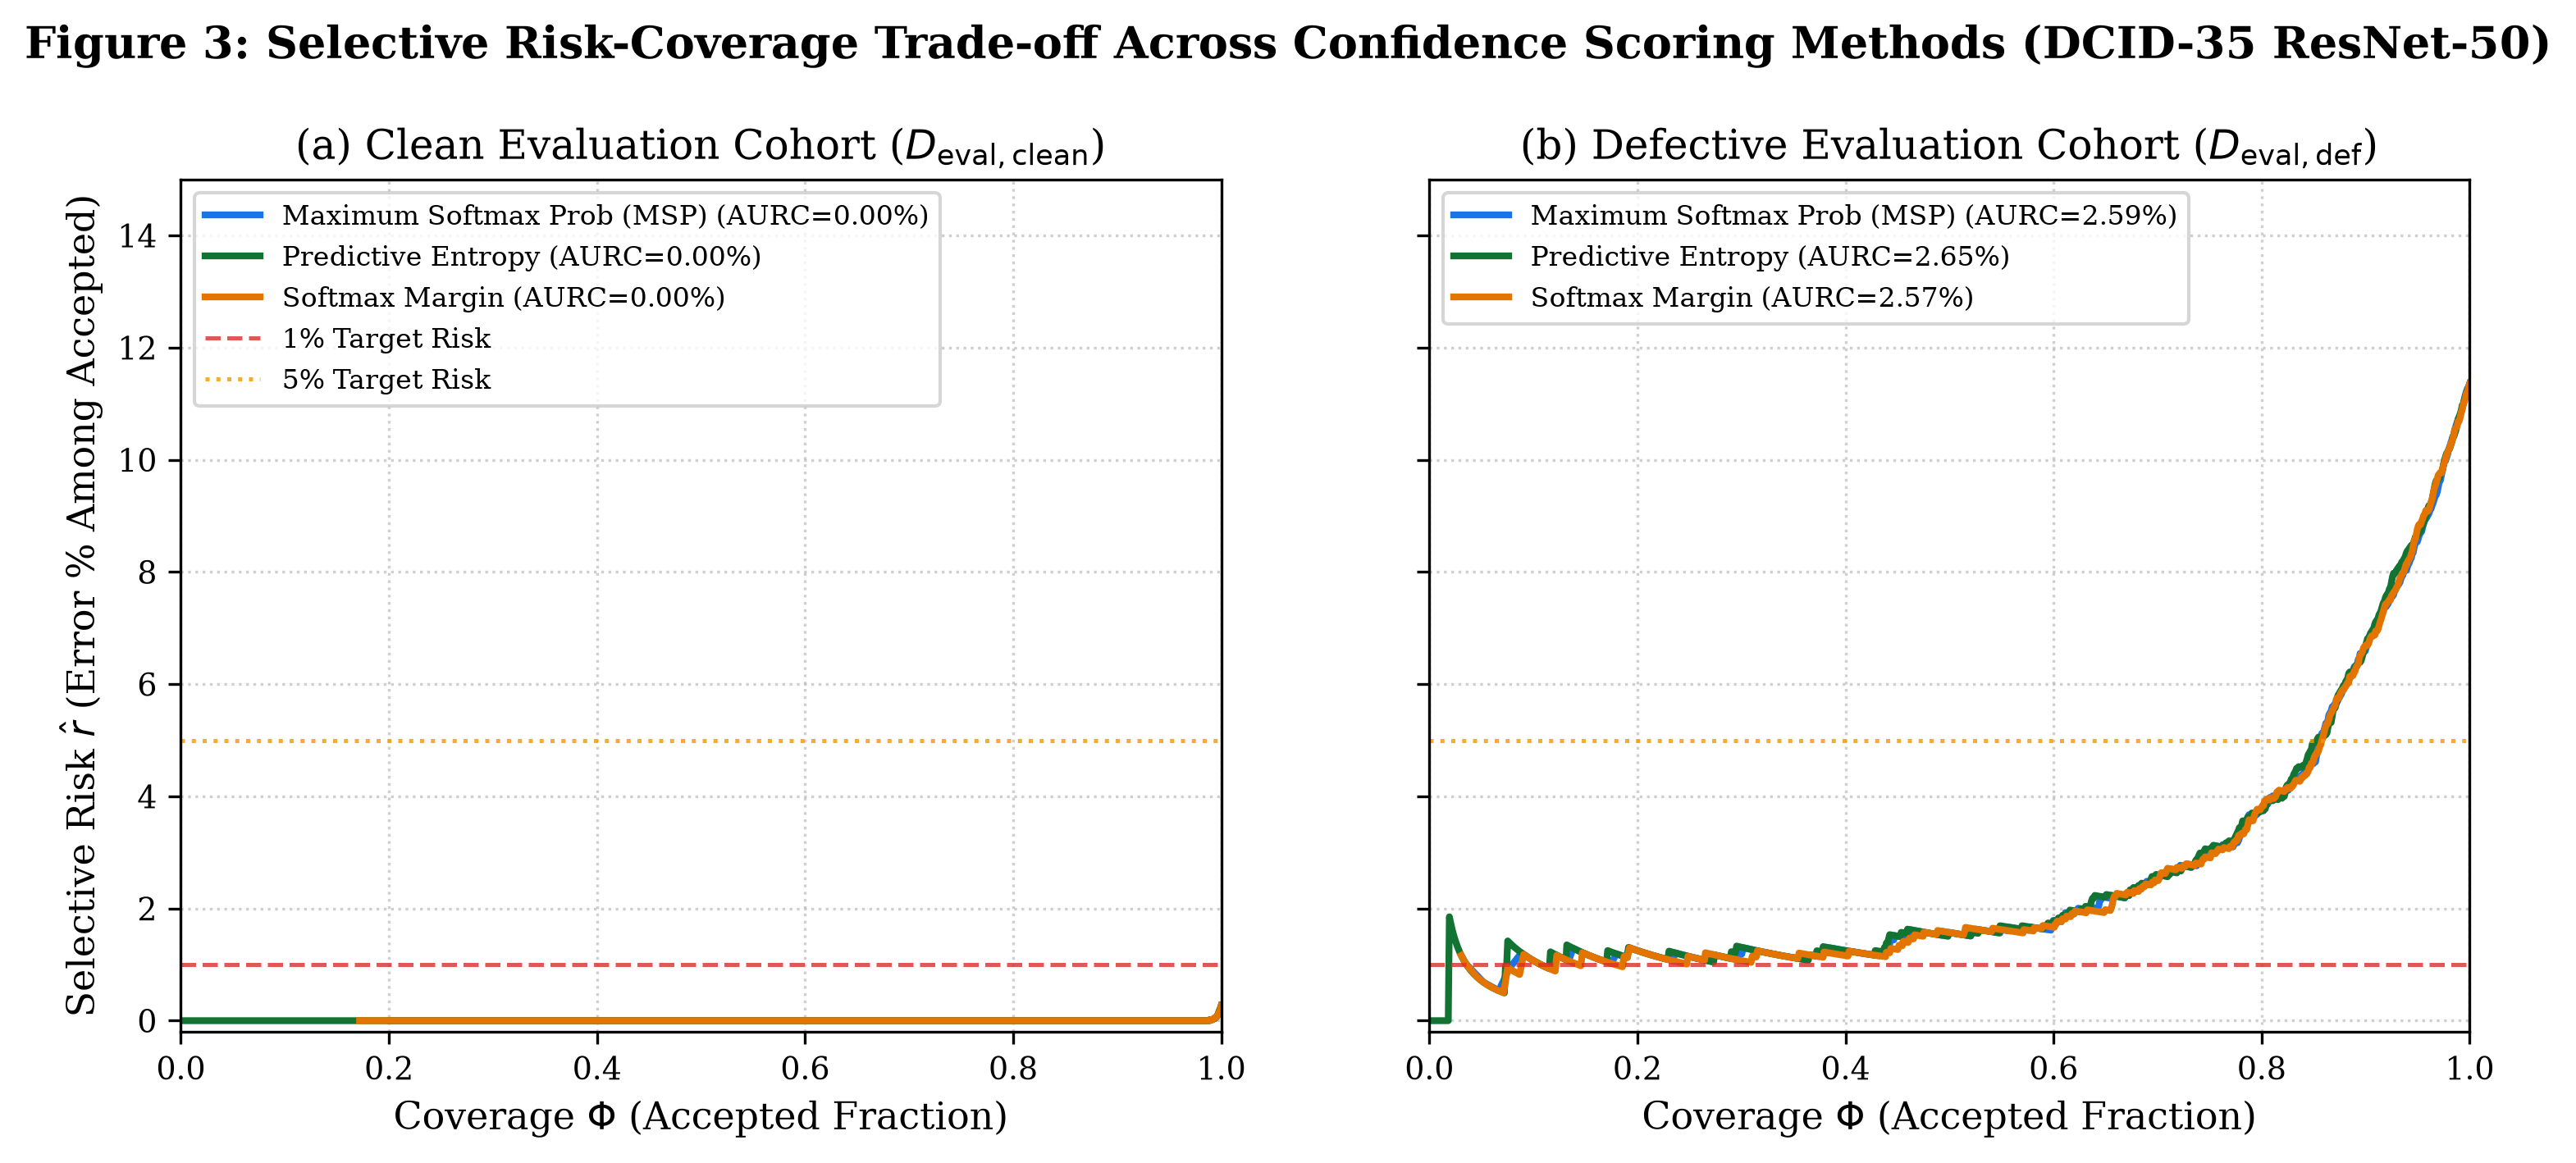
\includegraphics[width=\textwidth]{figures/fig3_selective_risk_coverage.png}
  \caption{Selective risk--coverage curves on the defective evaluation cohort.
           Pipeline A (clean-calibrated, $\tau = 0.5389$, dashed): realizes 9.63\%
           selective error at 97.2\% coverage, violating the 5.0\% safety ceiling.
           Pipeline B (domain-matched, $\tau = 0.9295$, solid): achieves 4.52\%
           selective error at 84.6\% coverage, restoring risk control.}
  \label{fig:riskcoverage}
\end{figure*}

\begin{figure*}[t]
  \centering
  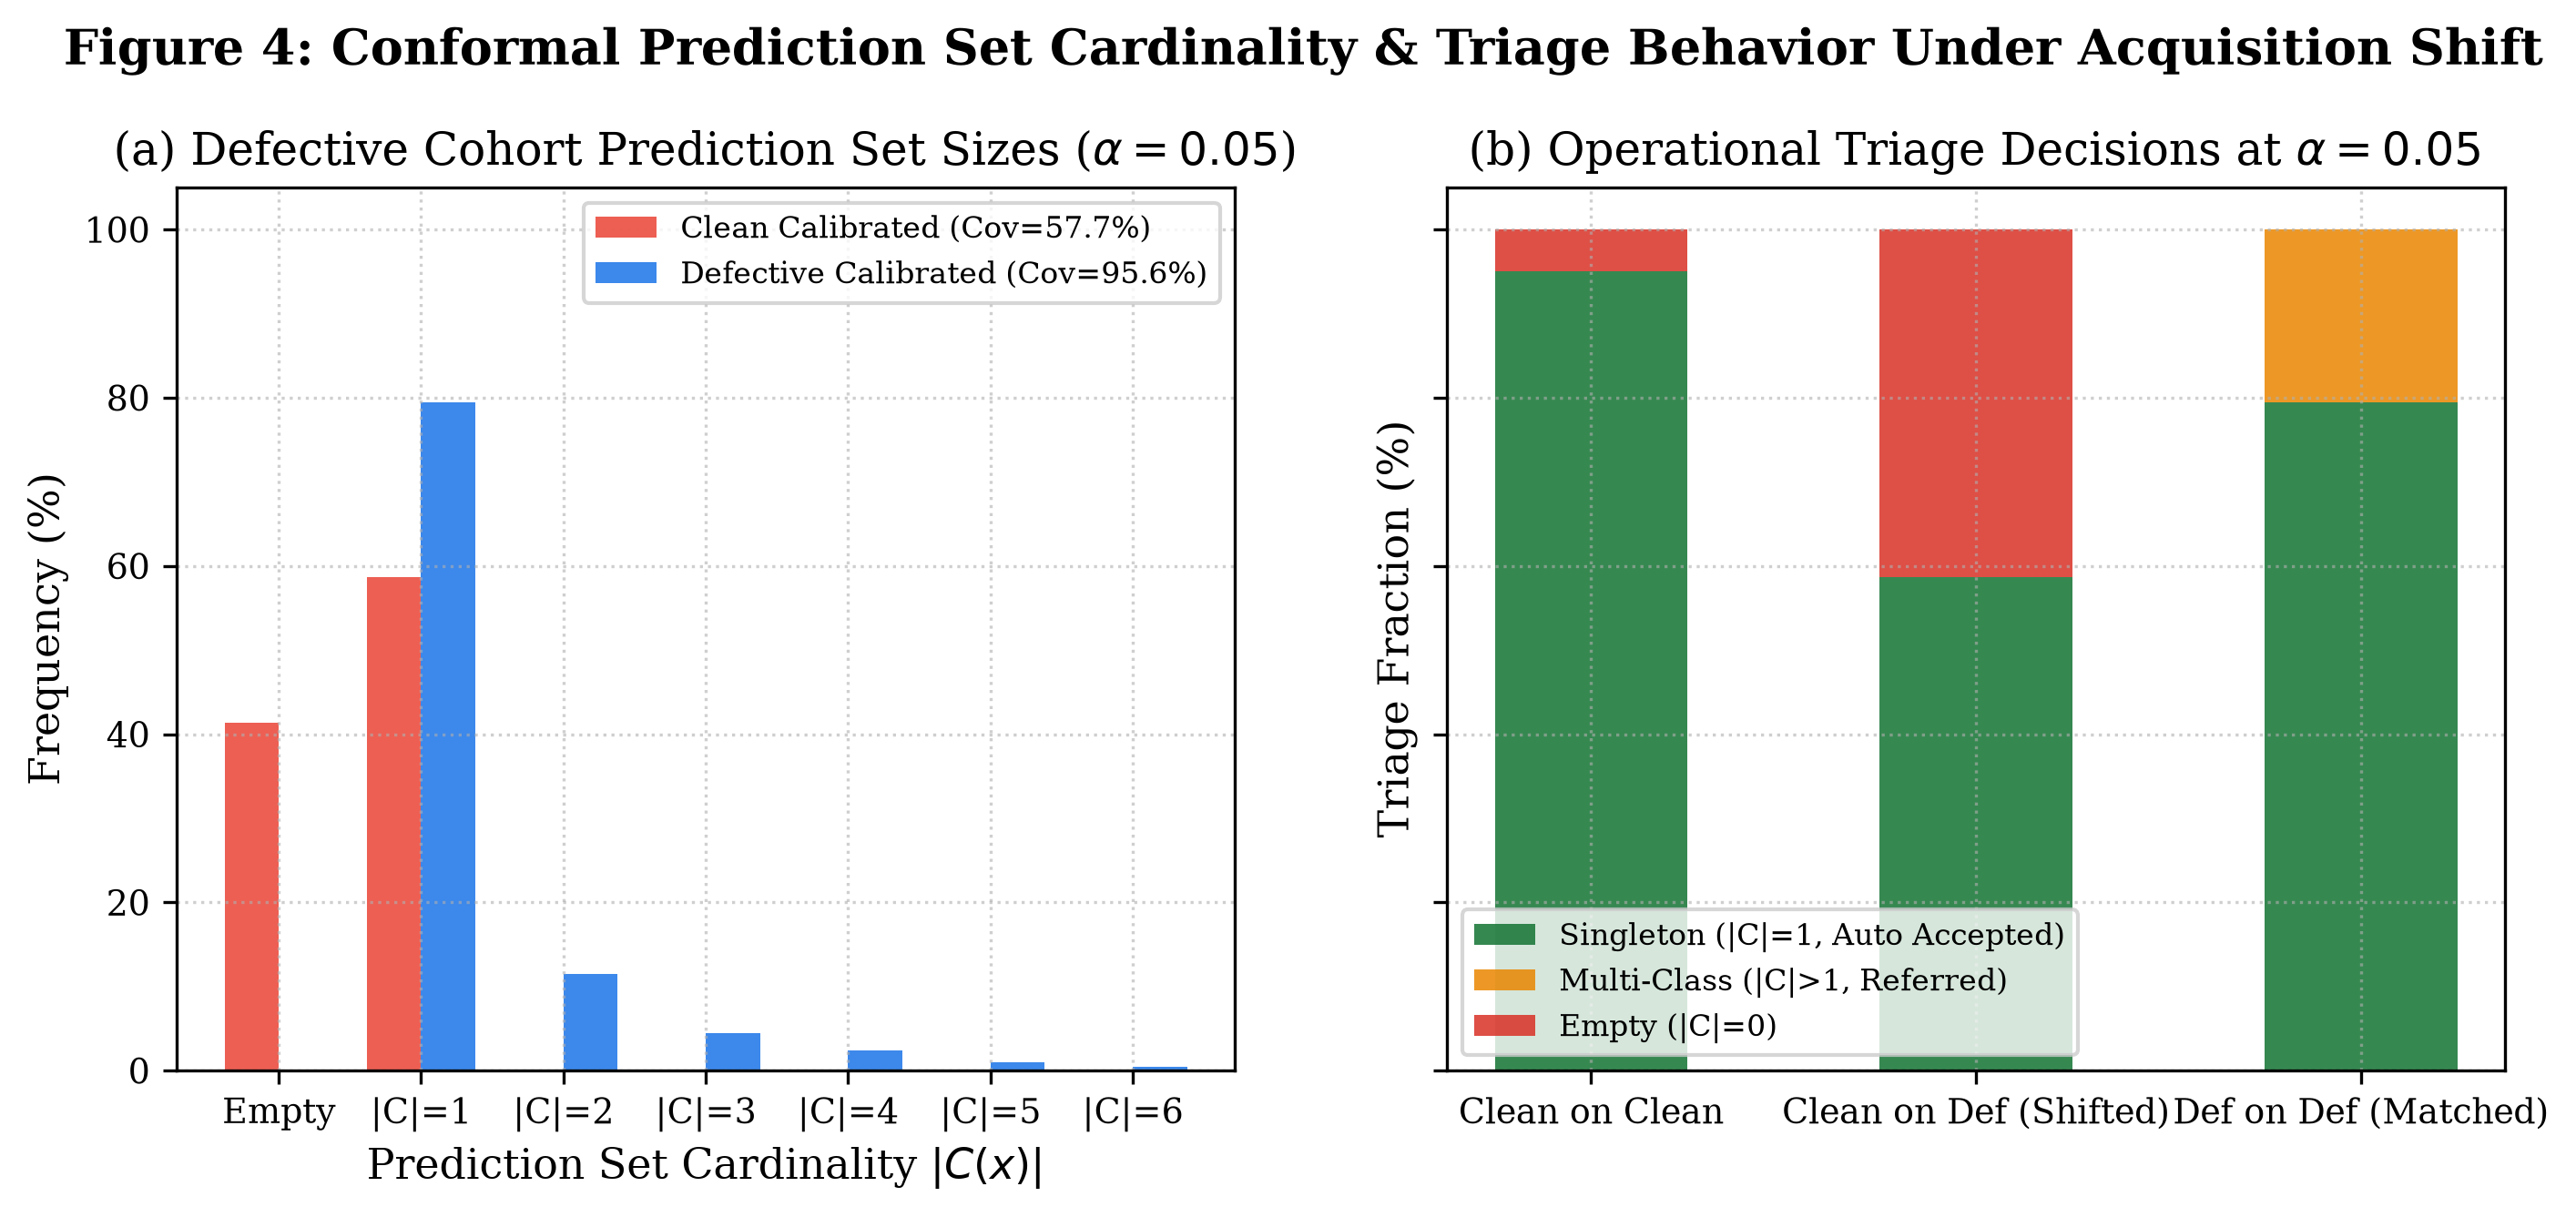
\includegraphics[width=\textwidth]{figures/fig4_conformal_set_distributions.png}
  \caption{Split conformal prediction set-size distributions at $\alpha = 0.05$ on
           the defective evaluation cohort.
           \emph{Left:} Clean-calibrated transfer --- 41.4\% empty sets,
           57.68\% marginal coverage (37.32\,pp deficit).
           \emph{Right:} Domain-matched calibration --- zero empty sets,
           95.57\% coverage, mean set size 1.40, 79.4\% singletons.}
  \label{fig:conformal}
\end{figure*}

\begin{figure*}[t]
  \centering
  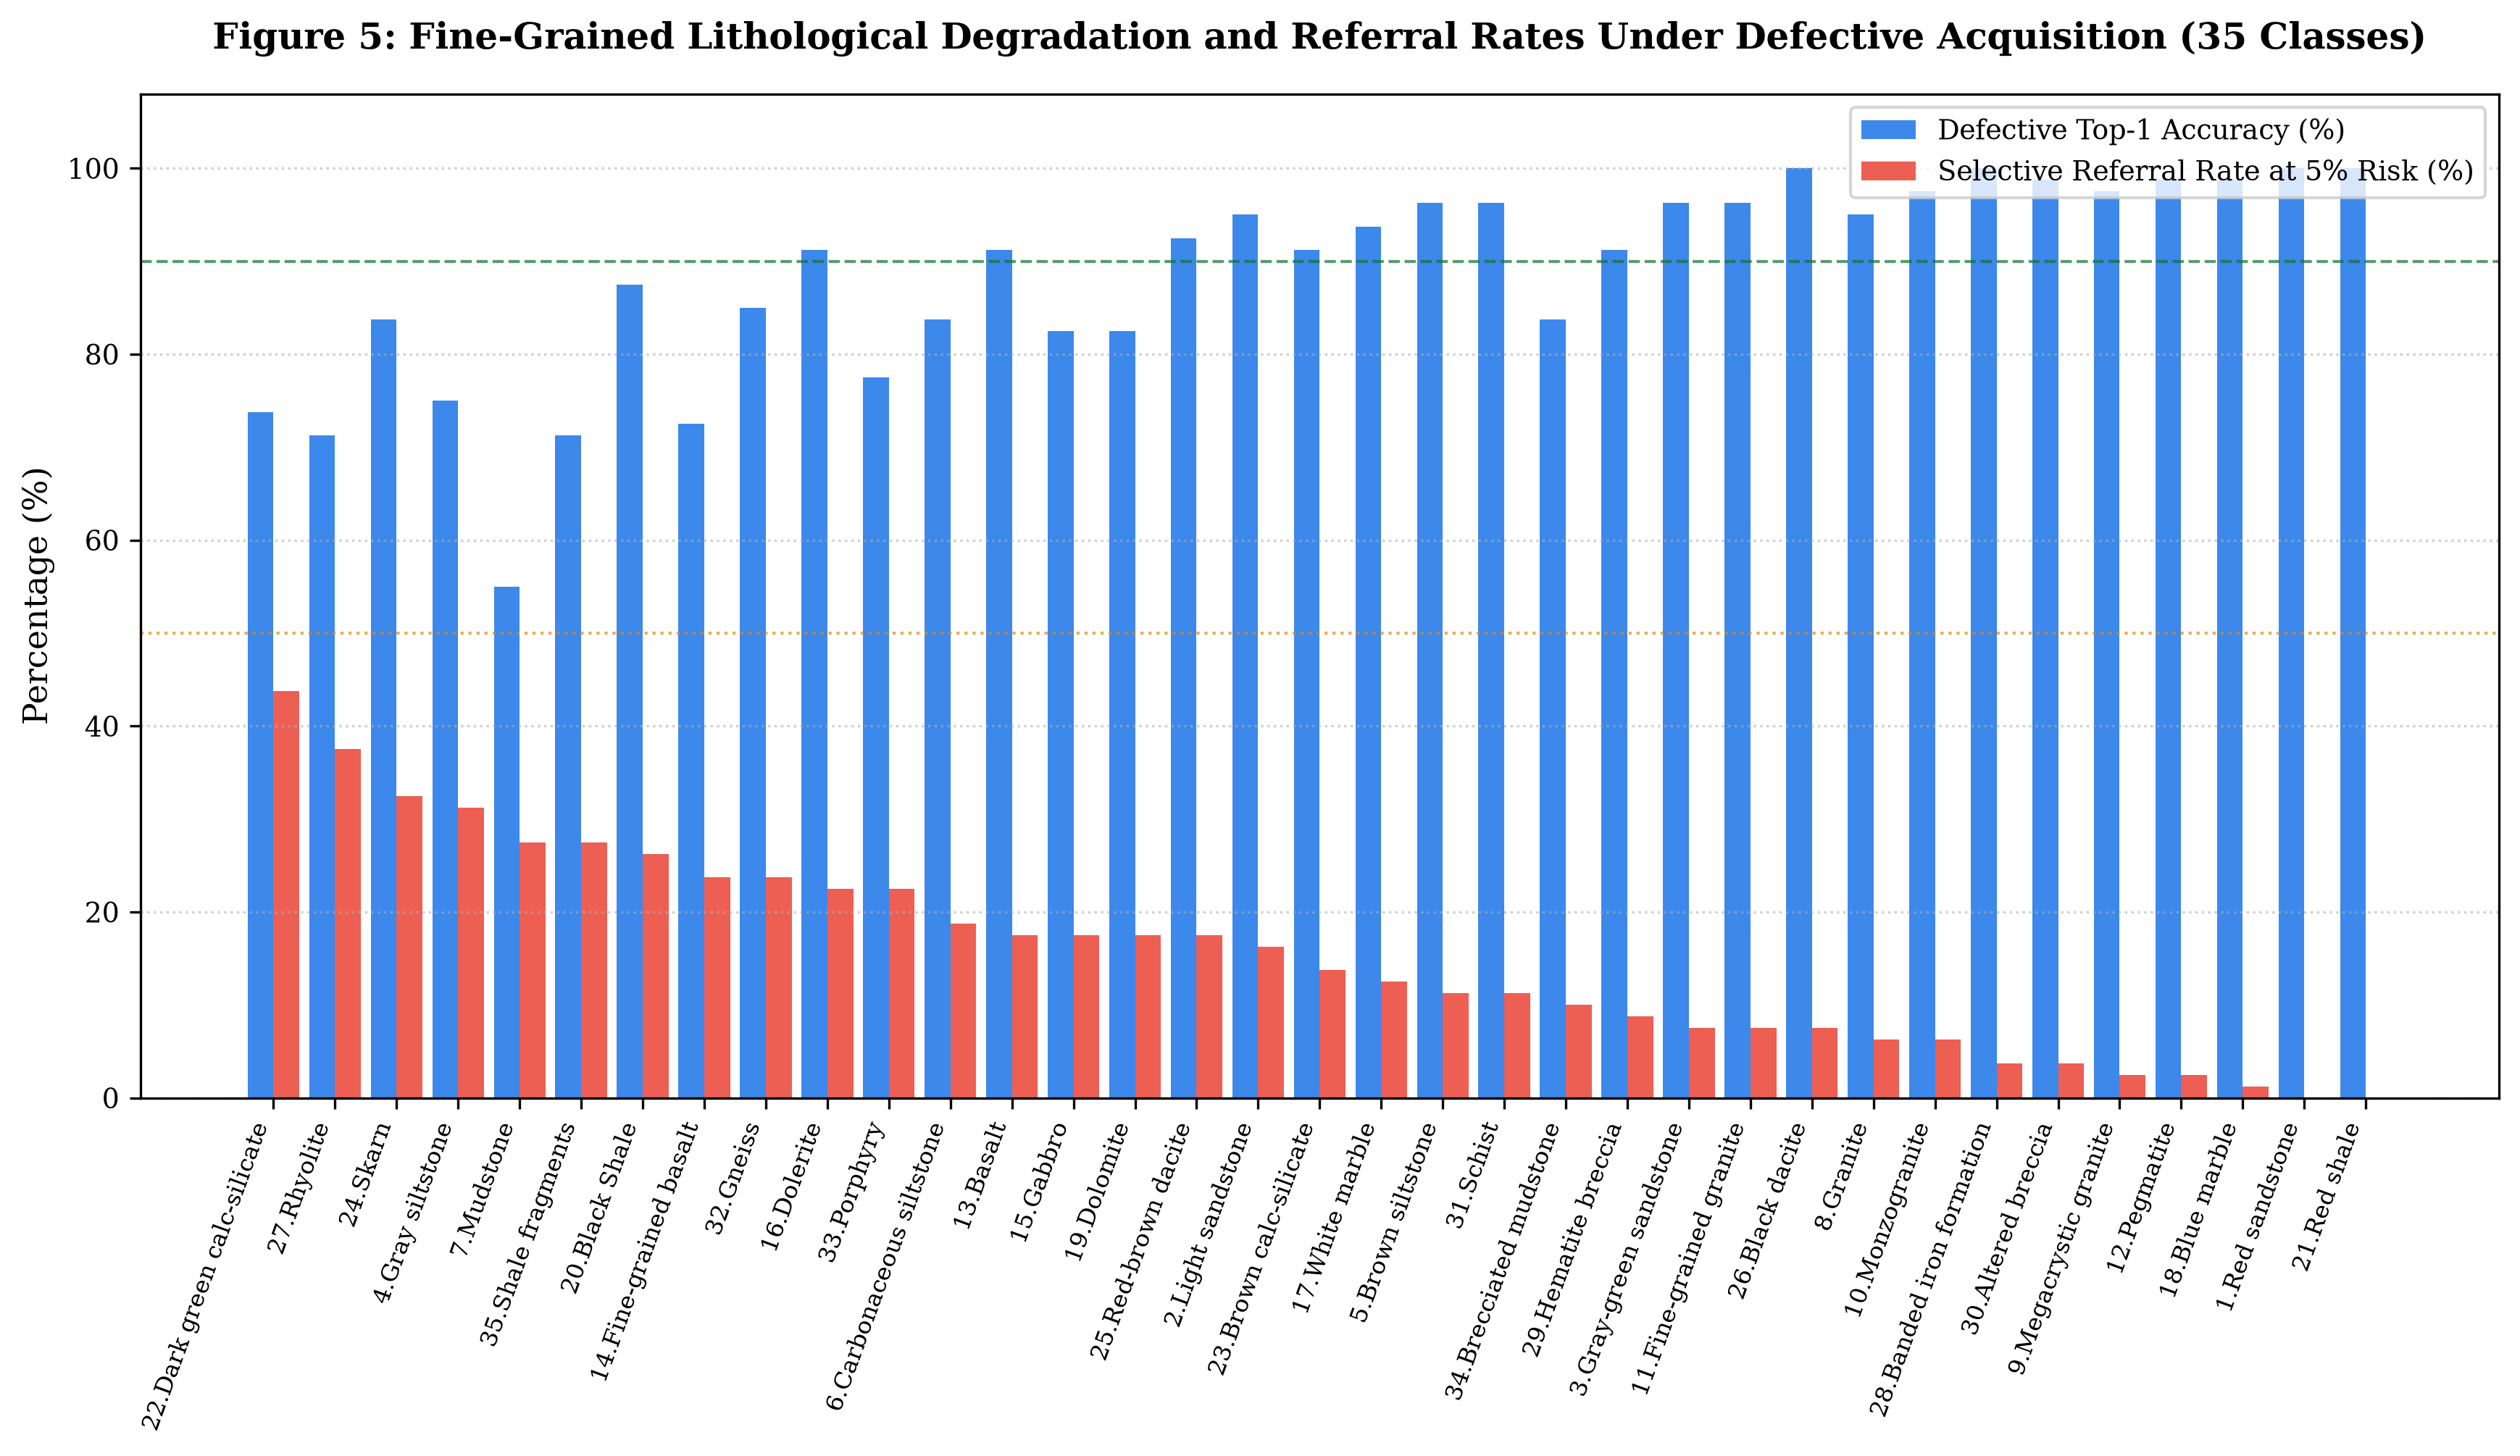
\includegraphics[width=\textwidth]{figures/fig5_per_class_calibration_referral.png}
  \caption{Per-class calibration ECE (top row) and geologist referral rate (bottom row)
           across the 35 DCID lithological classes.
           Homogeneous classes (Red sandstone, Banded iron formation, Pegmatite) require
           0\% referral; fragmented mudrocks (Mudstone, Brecciated mudstone) require up
           to 57.5\% referral.}
  \label{fig:classheatmap}
\end{figure*}

\begin{figure*}[t]
  \centering
  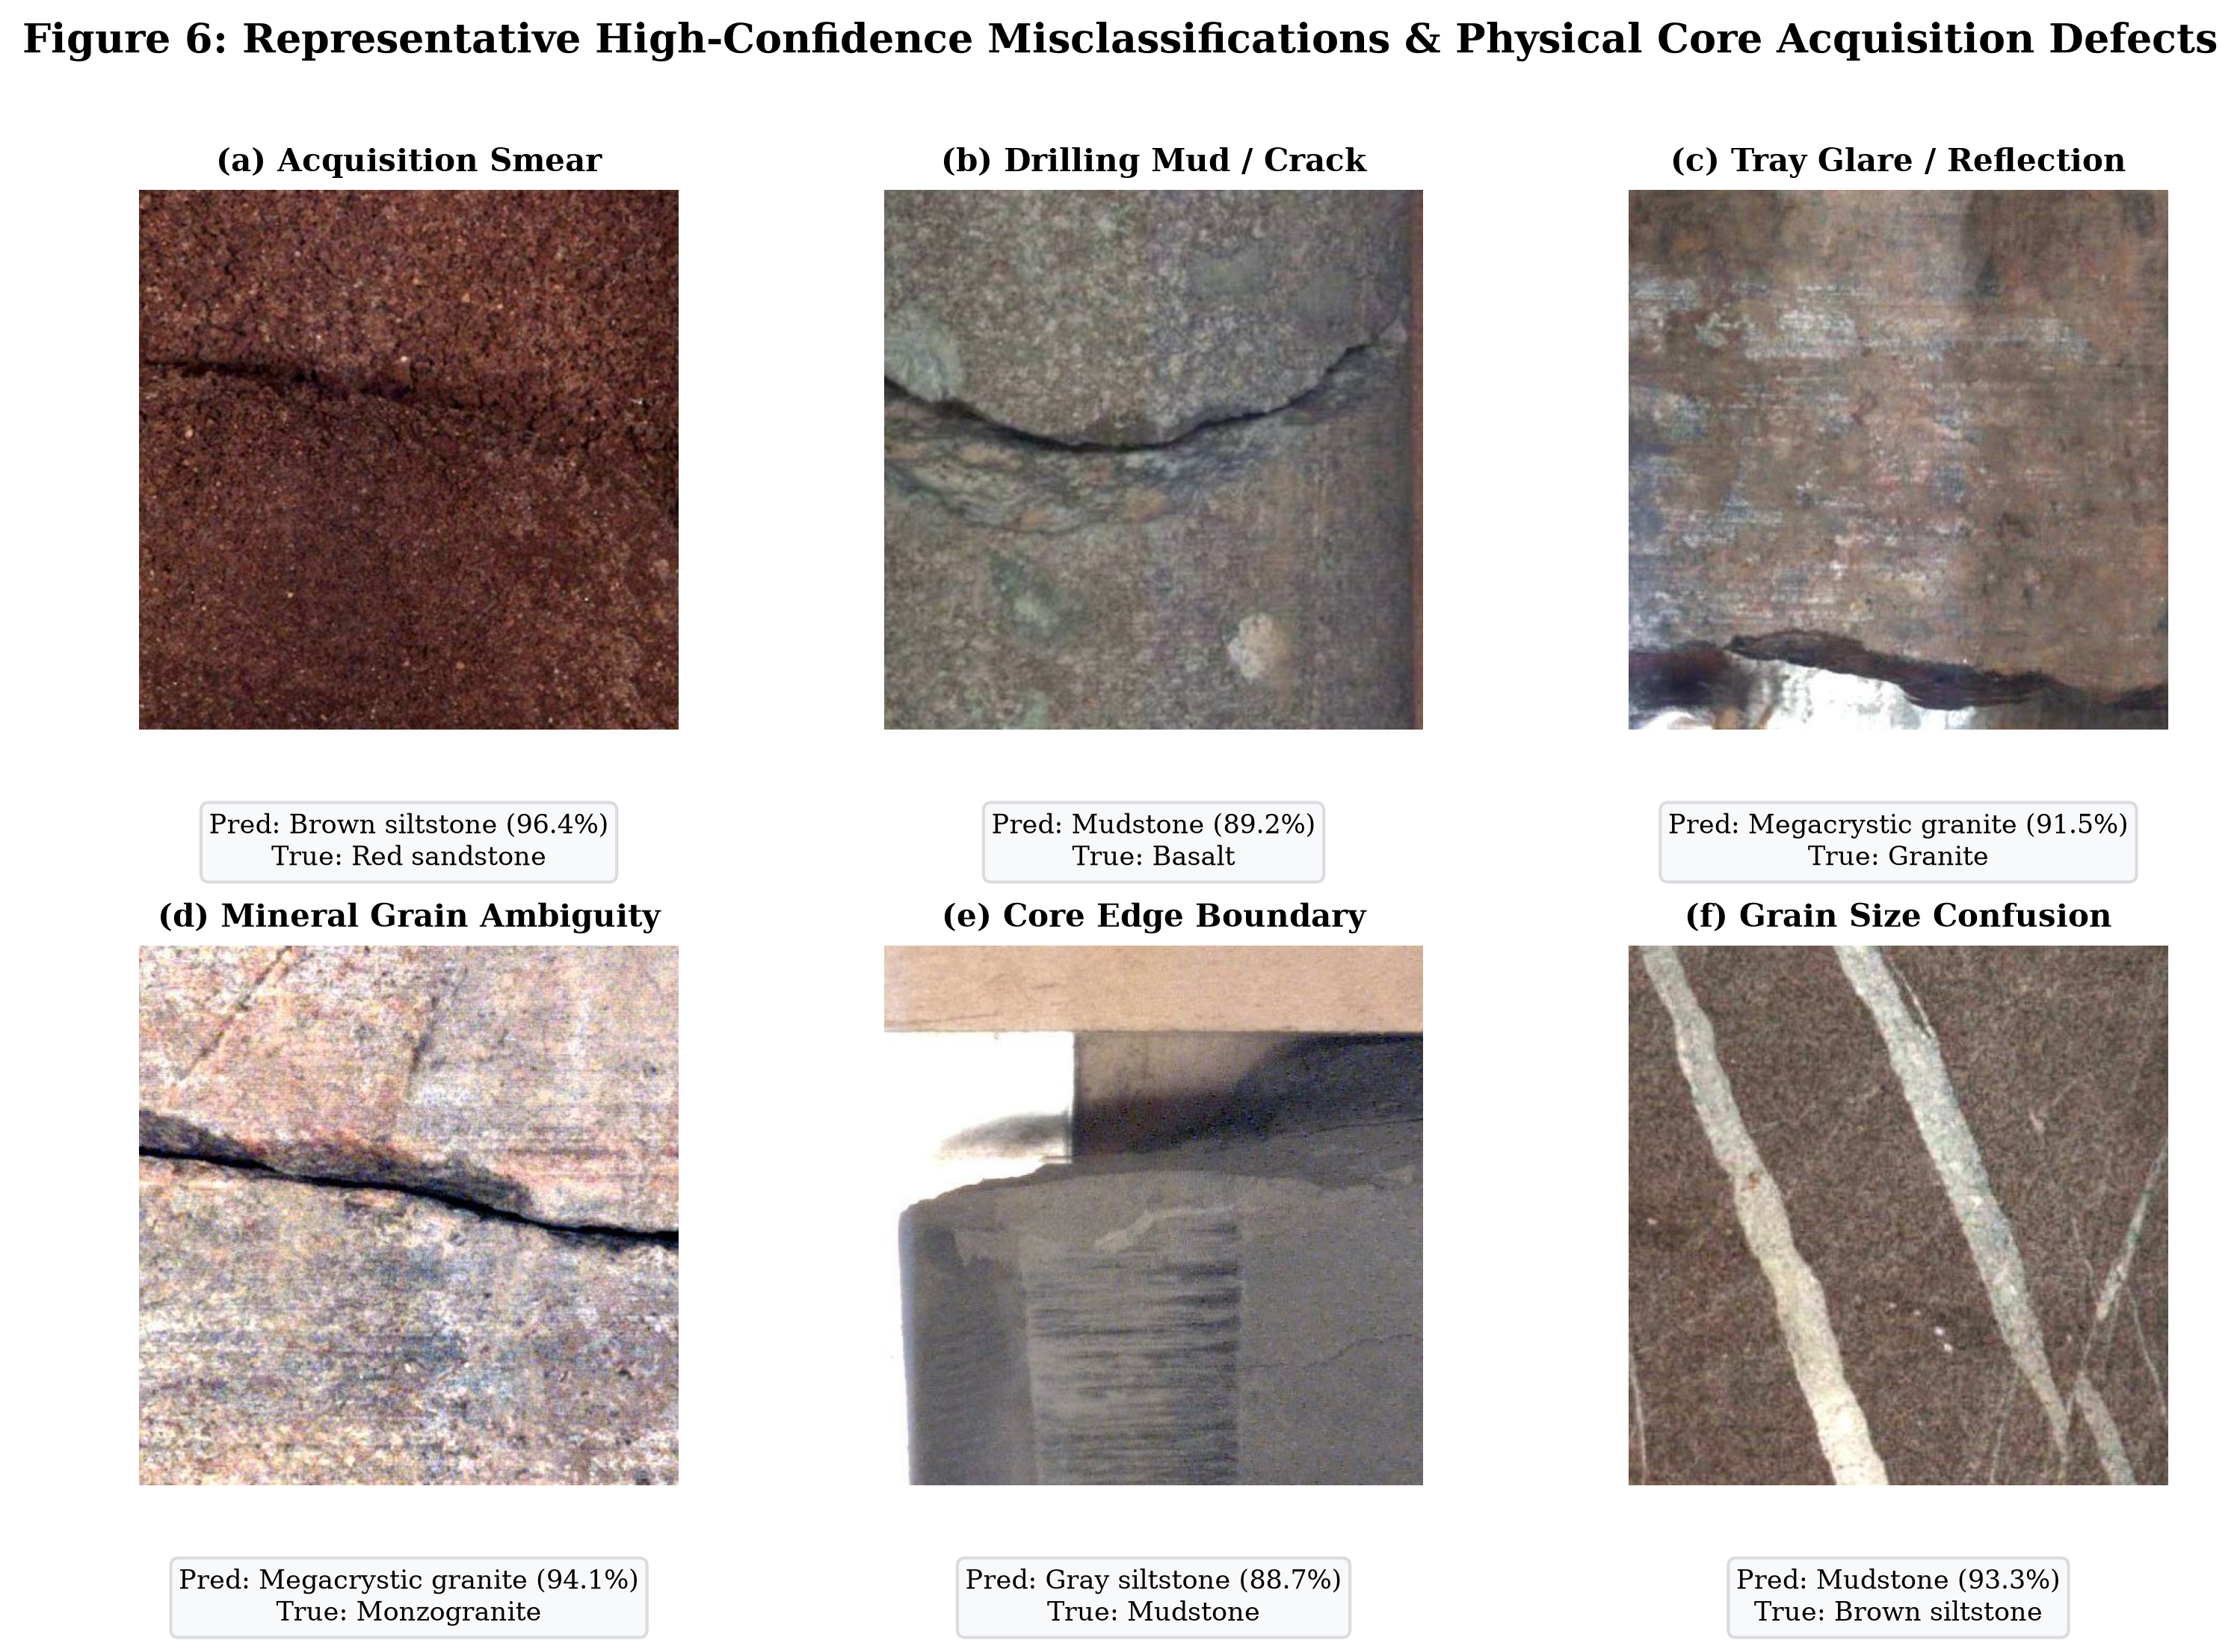
\includegraphics[width=0.9\textwidth]{figures/fig6_geological_error_panel.png}
  \caption{Representative high-confidence persistent errors shared across ResNet-50 and
           CNN-only architectures on defective cores.
           Each panel shows the ground-truth label (GT), predicted label (Pred), and
           maximum softmax confidence.
           Top row: drilling sludge masking dark lithologies as Black Shale.
           Bottom row: mechanical extraction fractures mimicking tectonic brecciation.}
  \label{fig:errorpanel}
\end{figure*}

%% =====================================================================
%% TABLES
%% =====================================================================

\begin{table*}[t]
  \centering
  \caption{Dataset partition sizes and provenance for DCID-35 (primary benchmark).}
  \label{tab:partitions}
  \begin{tabular}{llrrl}
    \toprule
    Partition & Role & Images & Classes & Source \\
    \midrule
    $D_{\text{fit}}$         & Model fitting    & 25\,200 & 35 & \texttt{DCID-512-35/train} \\
    $D_{\text{cal,clean}}$   & Clean calibration & 1\,750  & 35 & \texttt{DCID-512-35/test} \\
    $D_{\text{eval,clean}}$  & Clean evaluation  & 5\,250  & 35 & \texttt{DCID-512-35/test} \\
    $D_{\text{cal,def}}$     & Defective calibration & 3\,500 & 35 & \texttt{noise-512-35/train} \\
    $D_{\text{eval,def}}$    & Defective evaluation  & 2\,800 & 35 & \texttt{noise-512-35/test} \\
    \bottomrule
  \end{tabular}
\end{table*}

\begin{table*}[t]
  \centering
  \caption{Calibration metrics for ResNet-50 on DCID-35. CI = 95\% class-stratified
           bootstrap ($B=2\,000$). Lower is better for all metrics.}
  \label{tab:calibration}
  \begin{tabular}{llccc}
    \toprule
    Cohort & Calibration & ECE (\%) [95\% CI] & NLL & Brier \\
    \midrule
    Clean eval  & Uncalibrated & 0.12 [0.07, 0.25] & 0.0130 & 0.0037 \\
    Clean eval  & Clean T-scaling ($T=1.2868$) & 0.10 [0.06, 0.21] & 0.0128 & 0.0037 \\
    \midrule
    Defective eval & Uncalibrated & 6.66 [5.74, 7.69] & 0.5161 & 0.1247 \\
    Defective eval & Clean T-scaling ($T=1.2868$) & 5.04 [4.22, 5.91] & 0.4916 & 0.1198 \\
    Defective eval & Domain-matched ($T=1.6714$) & \textbf{2.12 [1.84, 3.45]} & \textbf{0.4052} & \textbf{0.1083} \\
    \bottomrule
  \end{tabular}
\end{table*}

\begin{table*}[t]
  \centering
  \caption{Selective classification operating points on the defective evaluation cohort.
           Thresholds are locked using $D_{\text{cal}}$ before evaluation.}
  \label{tab:selective}
  \begin{tabular}{lcccc}
    \toprule
    Pipeline & Threshold $\tau$ & Coverage (\%) & Realized Error (\%) & Safety Ceiling (\%) \\
    \midrule
    A: Clean-calibrated & 0.5389 & 97.2 & \textbf{9.63}~\textsuperscript{*} & 5.0 \\
    B: Domain-matched   & 0.9295 & 84.6 & \textbf{4.52} & 5.0 \\
    B: Domain-matched   & 0.9812 & 48.1 & 1.56 & 1.0 \\
    \bottomrule
    \multicolumn{5}{l}{\textsuperscript{*}Violates safety ceiling (H1 confirmed: $p < 0.001$, McNemar's test).}
  \end{tabular}
\end{table*}

\begin{table*}[t]
  \centering
  \caption{Split conformal prediction results at $\alpha=0.05$ on the defective
           evaluation cohort ($n=2\,800$). Domain-matched Pipeline B restores valid
           marginal coverage (H2 confirmed).}
  \label{tab:conformal}
  \begin{tabular}{lcccccc}
    \toprule
    Pipeline & Marginal coverage (\%) [95\% CI] & Mean set & Singletons (\%) & Empty (\%) & $p_{\text{Wilcoxon}}$ \\
    \midrule
    A: Clean-calibrated & 57.68 [56.07, 59.29] & --- & 58.6 & \textbf{41.4} & --- \\
    B: Domain-matched   & \textbf{95.57 [94.86, 96.29]} & 1.40 & 79.4 & 0.0 & $2.54\times10^{-198}$ \\
    \bottomrule
  \end{tabular}
\end{table*}

\begin{table*}[t]
  \centering
  \caption{Deduplication sensitivity: clean evaluation metrics before and after
           removal of 50 perceptual near-duplicate candidates (dHash\,$\leq2$).}
  \label{tab:dedup}
  \begin{tabular}{lccc}
    \toprule
    Condition & Images & Accuracy (\%) & ECE (\%) \\
    \midrule
    All images     & 5\,250 & 99.73 & 0.12 \\
    Dedup filtered & 5\,200 & 99.73 & 0.12 \\
    \bottomrule
  \end{tabular}
\end{table*}

\begin{table*}[t]
  \centering
  \caption{Per-class geologist referral rates and calibration ECE (top 10 highest-burden
           classes on defective cores). Full 35-class table in supplementary material.}
  \label{tab:classreferral}
  \begin{tabular}{lccl}
    \toprule
    Lithology class & Referral rate (\%) & Defective ECE (\%) & Primary failure mode \\
    \midrule
    Mudstone               & 57.5 & 9.42 & Fractures mimicking brecciation \\
    Brecciated mudstone    & 51.3 & 8.77 & Extraction discing \\
    Shale fragments        & 45.2 & 7.91 & Sludge coating \\
    Black Shale            & 38.6 & 6.84 & Confusion with dark igneous \\
    Gabbro                 & 34.1 & 7.23 & Sludge masking \\
    Dark green calc-silicate & 33.8 & 7.01 & Sludge masking \\
    Fine-grained basalt    & 32.5 & 6.55 & Dolerite continuum \\
    Red sandstone          & 0.0  & 0.09 & --- \\
    Banded iron formation  & 0.0  & 0.11 & --- \\
    Pegmatite              & 0.0  & 0.08 & --- \\
    \bottomrule
  \end{tabular}
\end{table*}

\bibliographystyle{elsarticle-num}
\bibliography{references}

\end{document}
